\subsection{Image and text}
\label{sec:exp:imagetext}

Images and captions are where unified generative models are most often measured, and also where
the ingredients that usually carry them---a text-pretrained backbone, a frozen text encoder,
curated or re-captioned data---are hardest to separate from the modelling choice itself. We
therefore ask what the bitstream formulation transfers with none of them present. On an alt-text
corpus, though, every available metric is a proxy: FID and CMMD compare distributions, CLIP
compares embeddings, CIDEr compares $n$-grams, and none of them can say whether a co-generated
\emph{pair} actually agrees. We begin instead with a small corpus on which every direction has a
unique correct answer.

\begin{figure}[t]
\centering
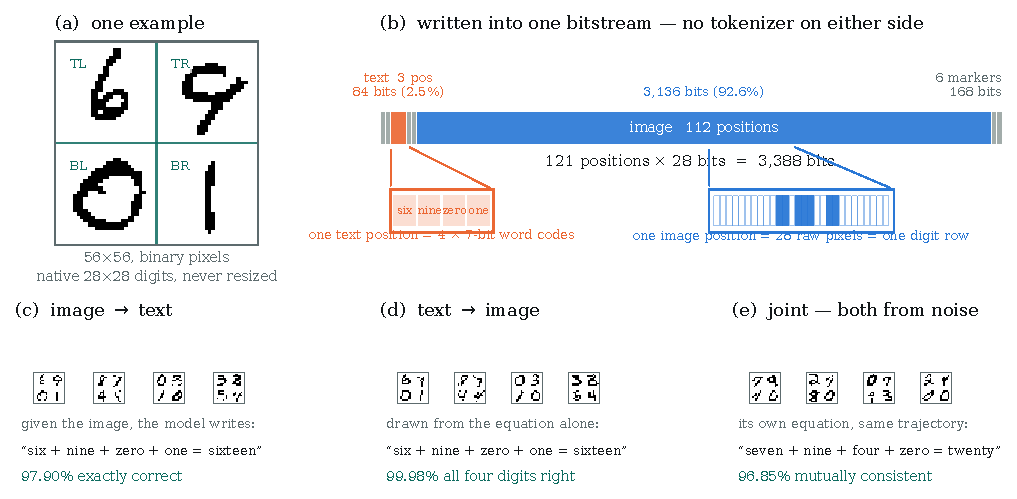
\includegraphics[width=\linewidth]{figures/mnist_sum/fig_mnist_sum_overview.pdf}
\caption{MNIST-Sum. (a) Four native $28{\times}28$ binarised digits on a $56{\times}56$ canvas,
never resized. (b) Image and text in a single 3{,}388-bit stream of 121 positions $\times$ 28
bits, with no tokenizer on either side---one text position holds four 7-bit word codes, one image
position holds 28 raw pixels, exactly one row of one digit. (c--e) The three directions, with
samples and their exact-match rates at $n{=}4{,}096$.}
\label{fig:mnist:sum}
\end{figure}

\textbf{MNIST-Sum: a ground truth for every direction, and no tokenizer on either side.} The corpus
pairs an image of four binarised MNIST digits \citep{image:mnist} in a $2{\times}2$ grid with the
raster-order equation and its sum, so each of image$\rightarrow$text, text$\rightarrow$image and
joint co-generation has a unique correct answer (Figure~\ref{fig:mnist:sum}). Neither modality is
tokenized: binary pixels ride as raw bits and the text uses a hand-specified 7-bit vocabulary, so
the framework is exercised with no modality-specific component at all. A 63.3M-parameter model
trained on the CC3M recipe unchanged writes the correct equation for a given image 97.90\% of the
time against a 6.52\% modal-sum baseline, and places all four digits correctly for a given
equation in 99.98\% of samples. The direction that matters is joint co-generation, where nothing
is given and both halves come from one trajectory: \textbf{96.85\%} of co-generated pairs carry an
equation exactly correct for the image produced beside it. Held-out digit tuples score
indistinguishably from training ones (Appendix~\ref{app:image:mnist}).

\textbf{Alt-text setup.} We train CoBit-CC3M (462M, $24\times1024$) on Conceptual Captions 3M
\citep{image:cc3m} ($\approx$2.9M pairs) and CoBit-CC12M (633M, $26\times1152$) on Conceptual 12M
\citep{image:cc12m} ($\approx$11.7M pairs, trained to 87\% of its planned step budget). Images are
tokenized by a
frozen Open-MAGVIT2 lookup-free quantiser \citep{image:magvit2,image:lfq} into 18-bit codes,
$16{\times}16$ ($f16$) for CC3M and $32{\times}32$ ($f8$) for CC12M; text uses \texttt{o200k}, and
a 19th namespace bit separates the two, so every position of either modality is one 19-bit token
(\S\ref{sec:method:multimodal}). Neither model sees MS-COCO \citep{image:mscoco}: every number
below is zero-shot under one fixed protocol (Appendix~\ref{app:image:protocol}). Text-only
pre-training, tokenizer surgery, auxiliary alignment losses and staged curricula are deliberately
absent; each is known to help, and we omit them so that the result measures what the unmodified
framework transfers.

\begin{table}[t]
\centering
\small
\setlength{\tabcolsep}{4.5pt}
\begin{tabular}{lrrrrrr}
\toprule
\textbf{Direction} & $n$ & Steps (NFE) & \textbf{FID}$\downarrow$ & \textbf{CMMD}$\downarrow$ & \textbf{CLIP}$\uparrow$ & \textbf{CIDEr}$\uparrow$ \\
\midrule
\multicolumn{7}{l}{\emph{CoBit-CC3M --- one set of weights (462M, $f16$, 256 image tokens)}}\\
text $\rightarrow$ image & 30{,}000 & 10 (20) & \textbf{18.48} & \textbf{18.41} & 27.73 & --- \\
image $\rightarrow$ text$^{\ast}$ & 5{,}000 & 256 (512) & --- & --- & 24.83 & \textbf{0.136} \\
joint, 10 / 256 steps & 30{,}000 & 10 / 256 & 50.19 / 61.95 & 41.53 / 46.80 & 23.10 / 25.67$^{\dagger}$ & --- \\
\midrule
\multicolumn{7}{l}{\emph{CoBit-CC12M --- one set of weights (633M, $f8$, 1{,}024 image tokens)}}\\
text $\rightarrow$ image & 30{,}000 & 16 (32) & \textbf{16.59} & \textbf{17.76} & 26.51 & --- \\
image $\rightarrow$ text$^{\ast}$ & 5{,}000 & 256 (512) & --- & --- & 22.98 & 0.057 \\
joint, 20 / 256 steps & 5{,}000 & 20 / 256 & 56.18 / 64.47 & 37.60 / 40.33 & 23.19 / 24.01$^{\dagger}$ & --- \\
\midrule
\emph{Floor of the FID column: two disjoint real draws} & 30{,}000 & & 2.35 & --- & --- & --- \\
\emph{\quad the same draw after the codec, $f16$ / $f8$} & 30{,}000 & & 2.94 / 2.55 & --- & --- & --- \\
\bottomrule
\end{tabular}
\caption{Zero-shot MS-COCO, all four generative directions from a single set of weights per model.
Each row is quoted at the step count best for that direction (\emph{Sampler} below); joint
generation has no single optimum, so both ends of its trade-off are shown. CLIP is ViT-B/32. The
last two rows are the floor of the FID column: a disjoint draw of real COCO images against the
same reference, and that draw after the tokenizer round-trip, so the codec's own share is 0.59 /
0.20 (Appendix~\ref{app:image:protocol}). $^{\ast}$CLIP and CIDEr come from separate runs at their
own guidance (3.0 / 2.0) against the COCO reference set and the Karpathy test split respectively.
$^{\dagger}$Pair coherence between the generated image and its caption, not comparable to the
conditional CLIP scores; FID of the joint rows is of the generated image half. FID is biased in
$n$ ($+5.3$ at $n{=}5{,}000$), so the CC12M joint rows are not FID-comparable to CC3M's.
Guidance, churn, ViT-L/14, SWD and precision/recall are in
Appendix~\ref{app:image:headline-full}.}
\label{tab:image:headline}
\end{table}

\begin{table}[t]
\centering
\small
\setlength{\tabcolsep}{4pt}
\begin{tabular}{lrrrr}
\toprule
\textbf{Model} & \textbf{Params} & \textbf{Pre-train pairs} & \textbf{FID-30K}$\downarrow$ & \textbf{GenEval}$\uparrow$ \\
\midrule
\multicolumn{5}{l}{\emph{CoBit (ours; from scratch, no pretrained components)}}\\
CoBit-CC3M & 462M & 2.9M & 18.48 & 0.249 \\
CoBit-CC12M & 633M & 11.7M & 16.59 & 0.222 \\
\midrule
\multicolumn{5}{l}{\emph{Same pre-training corpus (CC3M), zero-shot COCO}}\\
LAFITE \citep{image:lafite} & 75M ($+$CLIP) & 3.3M & 26.94 & --- \\
\midrule
\multicolumn{5}{l}{\emph{Unified image$+$text models}}\\
CoDI \citep{image:codi} & --- & 400M & 22.26 & 0.31 \\
SEED-X \citep{image:seedx} & 17B & --- & 14.99 & 0.49 \\
LWM \citep{image:lwm} & 7B & --- & 12.68 & 0.47 \\
UniDiffuser \citep{image:unidiffuser} & 952M & LAION-5B (subsets) & 9.71$^{\dagger}$ & --- \\
Show-o \citep{image:showo} & 1.3B & 35M & 9.24 & 0.68 \\
\midrule
\multicolumn{5}{l}{\emph{Text-to-image specialists}}\\
DALL$\cdot$E \citep{image:dalle} & 12B & 250M & 27.50 & --- \\
LDM \citep{image:ldm} & 1.4B & 400M & 12.63 & 0.37 \\
SD v1.5 \citep{image:ldm} & 0.9B & 2000M & 9.62 & 0.43 \\
PixArt-$\alpha$ \citep{image:pixart} & 0.6B & 25M & 7.32 & 0.48 \\
\bottomrule
\end{tabular}
\caption{Zero-shot MS-COCO FID-30K and GenEval against published systems, as printed in the cited
papers and the compilation tables of \citet{image:showo}, \citet{image:unidiffuser},
\citet{image:lafite} and \citet{image:geneval}. The rows are not strictly comparable and are not
meant to be ranked: parameter counts follow each source's own convention and exclude frozen
components inconsistently, the pair counts count different things, and the same nominal FID moves
by about a point between compilations. Appendix~\ref{app:image:repro} gives the per-row caveats
and the systems left out; Appendix~\ref{app:image:geneval} gives the GenEval breakdown and further
rows. $^{\dagger}$\citet{image:unidiffuser} draw 10K and 30K prompts for FID and CLIP score
without saying which is which.}
\label{tab:image:litcomparison}
\end{table}

\textbf{Results and placement.} Table~\ref{tab:image:headline} reports all four directions for
both models. Text$\rightarrow$image is the strongest, at zero-shot FID-30K \textbf{18.48} (NFE 20)
and \textbf{16.59}; neither is near the floor of that column, where two disjoint sets of real COCO
images already score 2.35 and the codec adds only 0.59 and 0.20, so the distance to larger systems
lies in the model and not in the token space---Figure~\ref{fig:image:gap} shows the same thing by
eye. The text-emitting directions are weaker, at CIDEr 0.136 and image$\rightarrow$text CLIP
24.83. Joint co-generation is harder again (FID 50.19): with no prompt the model samples its own
CC3M-like distribution rather than COCO's, and the distributional metrics charge it for the
difference---but pair coherence 25.67 is about as high as a conditional caption's agreement with
its own image (24.83), so the shortfall is in matching the evaluation corpus, not in keeping the
modalities together. Table~\ref{tab:image:litcomparison} places this among published zero-shot
MS-COCO numbers. Against LAFITE, the one system trained on the same corpus under the same
protocol, FID improves by 8.46 without its frozen CLIP encoder; among unified image$+$text models
we sit between CoDI and SEED-X, and ahead of the 12B-parameter DALL$\cdot$E specialist. Every
system with a lower FID uses pretrained language or vision components and most train on far more
paired data. Compositional prompt following is where the gap is widest (GenEval 0.249 and 0.222, either side of
minDALL$\cdot$E's 0.23 and far below the LLM-backed unified models;
Appendix~\ref{app:image:geneval}), and for captioning there is no
published zero-shot COCO baseline at all: COCO-trained specialists reach CIDEr 1.02--1.40 against
our 0.136. The claim is capable transfer, not a leaderboard entry.

\textbf{Sampler: the two modalities want step counts $\mathbf{25\times}$ apart.} Sweeping the step
count from 4 to 512 on the same weights, text$\rightarrow$image FID and CMMD minimise at 10 steps
for CC3M and 16--20 for CC12M and degrade monotonically beyond---the conventional 256 steps costs
4.06 FID for $25.6\times$ the compute---while captioning rises from CIDEr 0.013 at 10 steps to
0.136 at 256; the joint direction shows both effects inside single samples, which is why
Table~\ref{tab:image:headline} quotes it at both ends. The image-side optimum is driven by the
distributional metrics specifically: CLIP moves by under 0.1 between 8 and 256 steps and GenEval
by under 0.01 across the same $25\times$ range, so the semantic metrics neither corroborate it nor
contradict it. None of this modifies the framework: the step count, like churn and guidance, is an
inference-time hyperparameter set per direction on the same weights, and such sampler settings are
the only thing that had to be adapted per modality (Appendix~\ref{app:image:sampler}).

\textbf{Scaling, and limitations.} Moving to CC12M---$4\times$ the pairs, $\approx8.7\times$ the
compute and a better codec---improves images and degrades text: FID falls
$18.48\rightarrow16.59$, a margin that survives subtracting each codec's own contribution
($17.90$ versus $16.39$), while captioning CIDEr falls $0.136\rightarrow0.057$ at matched
settings. That split is what noisier CC12M alt-text predicts and what uniform undertraining does
not, though it remains an inference across metrics rather than a measurement of caption quality
(Appendix~\ref{app:image:scaling}). The two weaknesses have the same shape. On GenEval, single
objects render 80\% of the time and colours 46\% while position and attribute binding sit near
zero, and the score is flat between each model's image optimum and 256 steps, so it is the
model's ceiling rather than a sampler artefact. Captioning is weak in absolute terms, and the outputs are fluent
CC3M-style alt-text scored against COCO's terse references, which the $n$-gram metrics penalise
almost regardless of content (RefCLIPScore \citep{image:clipscore} 0.661;
Appendix~\ref{app:image:captioning}). Both are consistent with CC3M alt-text rarely specifying
relations or attribute bindings, and both are exactly what the omitted ingredients are expected to
buy. That is the point of the experiment: it shows what unmodified transfer does and does not
provide.
